\documentclass[a4paper]{article}
\usepackage[utf8]{inputenc}
\usepackage{draculatheme}
\usepackage{graphicx}
\usepackage{color}
\usepackage{nopageno}
\usepackage{fontawesome}
\usepackage{listings}
\usepackage[export]{adjustbox}
\usepackage[fontsize=8pt]{fontsize}
\usepackage{titlesec}
\usepackage{hyperref}


\usepackage[a4paper, total={7.8in, 11.5in}]{geometry}
\graphicspath{ {./images/} }
\title{Project 4 Submission}
\author{Chaitanya Sharma}
\date{March 2023}

\newcommand*{\xdash}[1][3em]{\rule[0.5ex]{#1}{0.55pt}}

\makeatletter
\renewcommand\paragraph{\@startsection{paragraph}{4}{\z@}%
% display heading, like subsubsection
                                     {-3.25ex\@plus -1ex \@minus -.2ex}%
                                     {1.5ex \@plus .2ex}%
                                     {\normalfont\normalsize\bfseries}}


\renewenvironment{abstract}{%
    \if@twocolumn
      \section*{\abstractname}%
    \else 
      \begin{center}%
        {\bfseries \Large\abstractname\vspace{\z@}}
      \end{center}%
      \quotation
    \fi}
    {\if@twocolumn\else\endquotation\fi}

\setcounter{secnumdepth}{4}

\makeatother
\begin{document}
\begin{center}
	\begin{abstract}
		This is the design document of Chaitanya Sharma for Project 4 for ECE 250's Winter 2023 offering.
	\end{abstract}
\end{center}


\section{Introduction}
	My program consists of a major class {\color{draculapurple}PowerGridGraph}, and one nested class inside that, namely {\color{draculapurple}EdgesPriorityQueue}.
	My code has three macro functions(preprocessor directives) which are used to declare the left and right child and the parent of a node in the priority queue minimum heap.

	I attribute the latex template which I've used for this design document to myself as I've used it in the past for my other projects in this course.

	I've tested all edge test cases possible and also used the test cases provided by the
	jekelautograder on {\color{DarkPastelBlue}https://github.com/JZJisawesome/ece250-testcases}.
\newline

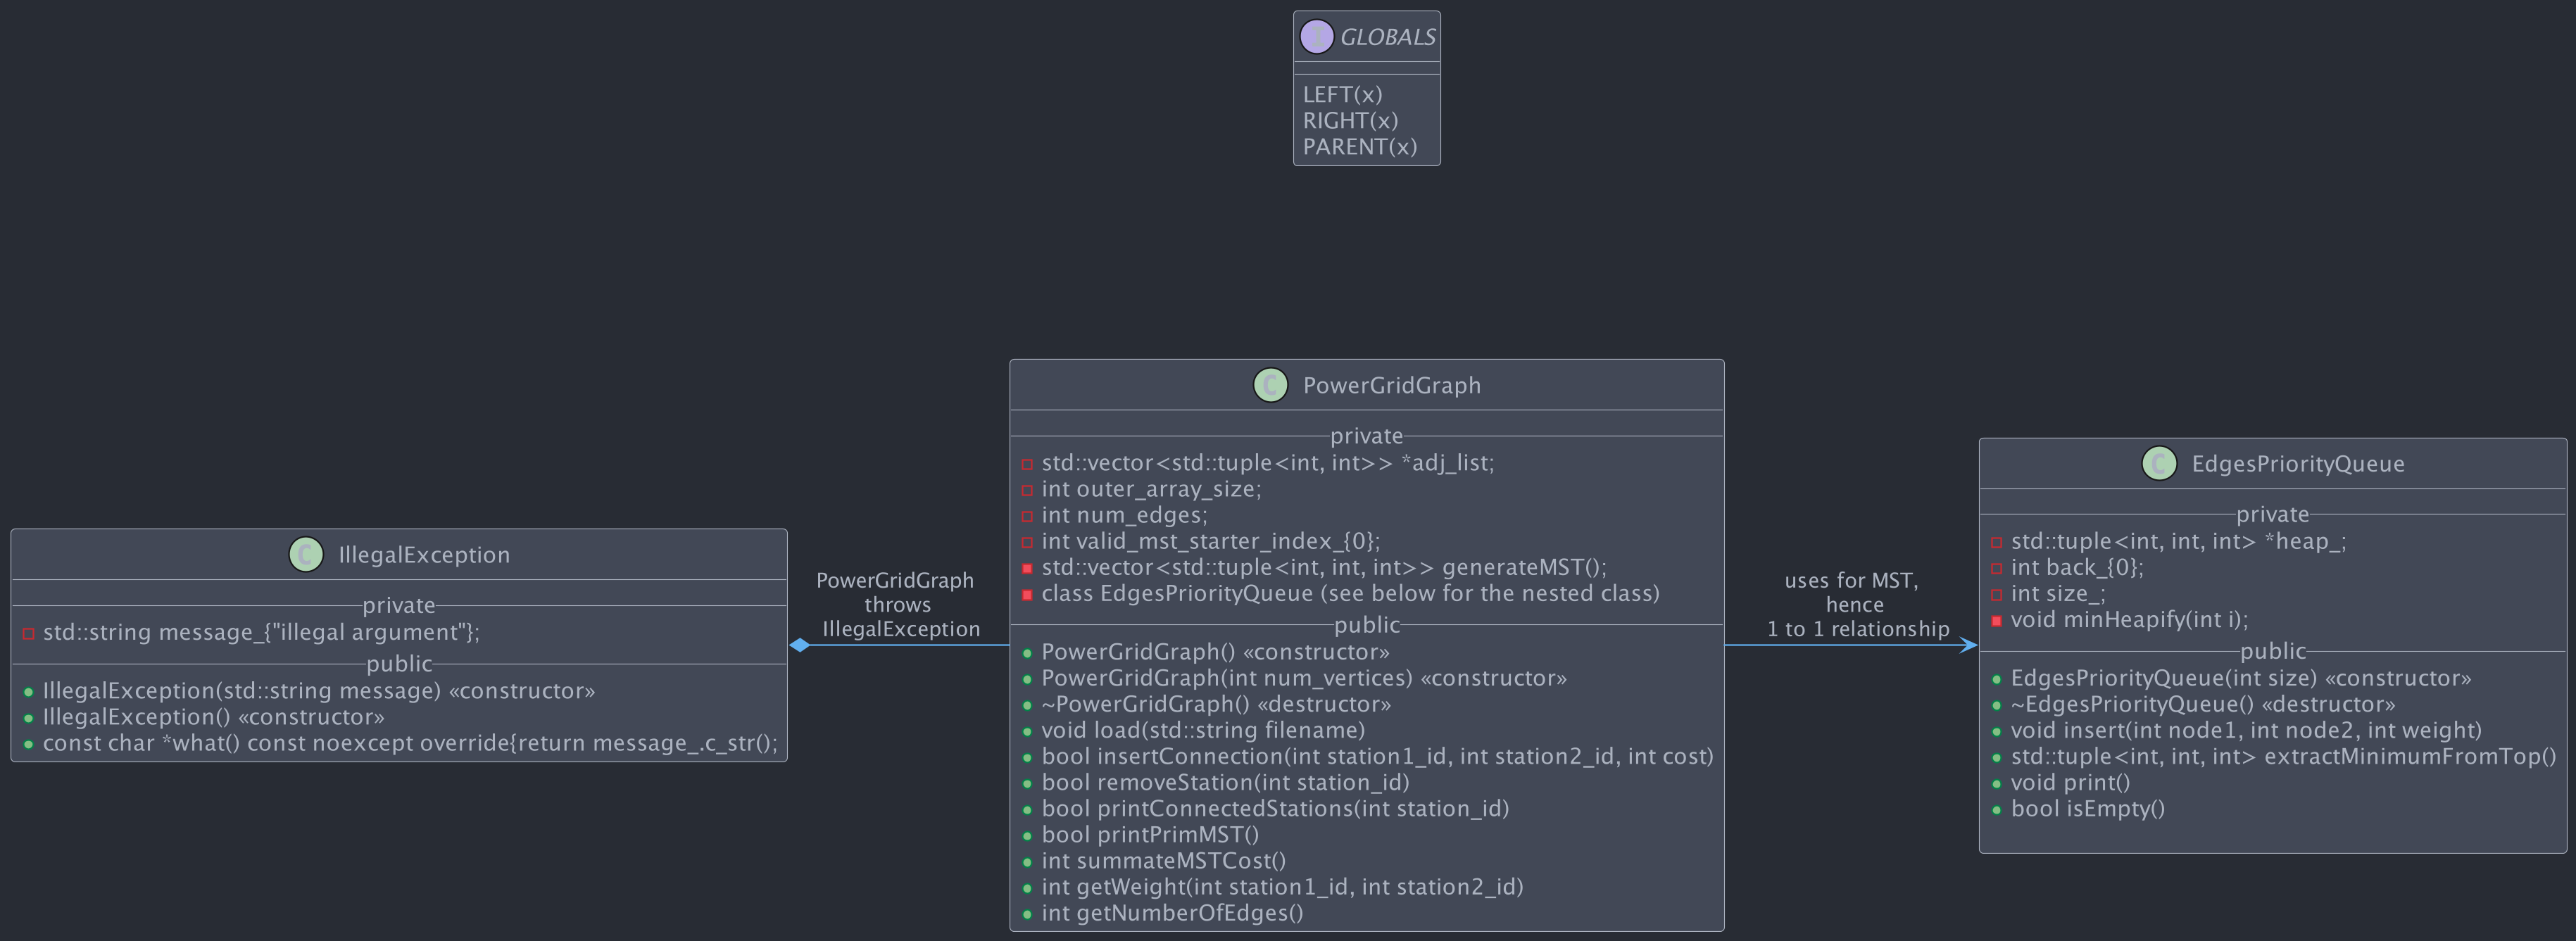
\includegraphics[scale=0.145, center]{PowerGridGraph.png}

\section{Class Structure}
	\subsection{{\color{orange}class} {\Large{\color{draculapurple}IllegalException}}}

		I attribute this class to myself as I've used it in the past for my other previous projects in this course.
		I'm using a default constructor and a parameterized constructor for this class. Though I'm not using the 
		parameterized constructor in my code, I've included it for future use.
		This is a simple exception class which I've inherited from the {\color{draculapurple}std::exception} class. 
		It has a private member variable {\color{Turquoise}message\_} which is a string which stores the message to be 
		displayed when the exception is thrown. It has a constructor which takes a string as an argument and assigns it 
		to the {\color{Turquoise}message\_} variable. It also has a default constructor which assigns the default 
		message to the {\color{Turquoise}message\_} variable. It has a {\color{draculapurple}what()} function which returns 
		the {\color{Turquoise}message\_} variable as a {\color{draculapurple}const char*}.


	\subsection{{\color{orange}class} {\Large{\color{draculapurple}PowerGridGraph}}}

		This class represents the whole power grid graph. It has a private member variable {\color{Turquoise}adj\_list} which is a 
		dynamically allocated array of {\color{draculapurple}std::vector} of {\color{draculapurple}std::tuple} of dual {\color{draculapurple}int}s.
		The other important private member variable is {\color{Turquoise}num\_edges} which stores the number of edges in the graph, 
		and the {\color{Turquoise}outer\_array\_size} which stores the size of the static {\color{Turquoise}adj\_list} array.

		There's also a {\color{Turquoise}valid\_mst\_starter\_index\_} private member variable which is used to keep track of the 
		{\color{draculapurple}int} index of the {\color{Turquoise}adj\_list} array which is the starting point of the MST generation.
		This lets me start the MST generation from any arbitrary node with more than 0 edges, and not just from the first node in the 
		{\color{Turquoise}adj\_list} array which just couldn't just be there in some cases. The alternative to this would be to run a for loop at time of 
		{\color{draculapurple}generateMST}() function call to find the first node with more than 0 edges, but that would be a waste of time as well as ruin the time complexity of my 
		{\color{draculapurple}generateMST}() function. The value of this private member variable is maintained appropriately by {\color{draculapurple}insertConnection}() and 
		{\color{draculapurple}removeStation}() functions.

		This class has two constructors which are the default constructor and the value init constructor which takes in a single 
		{\color{draculapurple}int} as an argument, and dynamically allocates the {\color{Turquoise}adj\_list} array with the size.
		It also has a destructor which deallocates the {\color{Turquoise}adj\_list} array, to make the program memory safe.

		\begin{center}
			\noindent\hrulefill\raisebox{-.3\ht\strutbox} { {\textbf{\Large{Graph's Private Member Functions And Classes}}} } \hrulefill\par
		\end{center}

		\subsubsection{{\color{orange} std::vector<{\color{azure}EDGE}> } {\color{draculapurple}generateMST}()}

			This function is used to generate the minimum spanning tree. It first checks if the number of edges is 0, and if it is, it returns an empty vector of tuples.
			Then it creates a boolean array of size {\color{draculapurple}outer\_array\_size} and initializes all the values to {\color{draculapurple}false}.
			I treat the boolean array as a set to check if a vertex has been visited or not in {\color{lightblue}O(1)} time, and set all of them to false.
			
			Then this function creates a vector of triple int tuple, which will represent our final product, the minimum spanning tree of the graph.
			Then it creates a pointer to an object of the {\color{draculapurple}EdgesPriorityQueue} class, with its size init constructor of the size of the number of edges.
			Then it creates a random index for the starting vertice of the minimum spanning tree, and sets the value of the boolean array at that index to {\color{draculapurple}true}.
			This random index is assigned to the {\color{Turquoise}valid\_mst\_starter\_index\_} private member variable of the {\color{draculapurple}PowerGridGraph} class.
			What this random index is determined by the {\color{draculapurple}insertConnection} function and the {\color{draculapurple}removeStation} function.
			Then it iterates through the adjacency list of the random index, and inserts the values of the tuple in the priority queue.
			Then it enters a while loop which runs until the priority queue is empty, and in each iteration, it extracts the minimum element from the priority queue, and stores it in a tuple.

			The time complexity of Prim's algorithm is {\color{lightblue}O(|E|log(|V|))}, where {\color{draculapurple}|E|} is the number of edges and 
			{\color{draculapurple}|V|} is the number of vertices in the graph.
			In this function, the number of edges is given by the variable {\color{draculapurple}num\_edges}, which is used to create the priority queue 
			with an initial capacity of {\color{draculapurple}num\_edges}. The size of the priority queue can increase up to {\color{draculapurple}|E|} 
			during the algorithm execution, but its maximum size is {\color{lightblue}O(|E|)} because each edge can be inserted and extracted at most once.
			The while loop iterates until the priority queue is empty, which takes {\color{lightblue}O(|E|log(|E|))} time because each insertion and 
			extraction operation takes {\color{lightblue}O(log(|E|))} time.
			Inside the while loop, there are two for loops that iterate over the adjacent vertices of the current minimum edge. The total number of 
			iterations of these for loops is at most {\color{draculapurple}2|E|}, because each edge is visited twice (once for each adjacent vertex) at most.
			Therefore, the overall time complexity of this function is {\color{lightblue}O(|E|log(|E|) + 2|E|) = O(|E|log(|E|))}.
			However, the number of edges {\color{draculapurple}|E|} may be proportional to the number of vertices {\color{draculapurple}|V|} in the worst
			 case (e.g., for a complete graph), so the time complexity can also be expressed as {\color{lightblue}O(|E|log(|V|))}.
			 
			 Also, a good thing about my implementation is that, while researching about Prim's algorithm, I found out that a lot 
			 of people implement a hash table to find the home node for a given edge along with the priority queue, but what I did was while inserting into my 
			 priority queue and making it, I just stored the home node in the tuple itself, and that saved me a lot of time and space complexity allowing me to find the home node in 
			 {\color{lightblue}O(1)} time.
			 
			 {\color{GoldenYellow}"MST"} {\color{GoldenYellow}"COST"} {\color{pink}common function}

		\subsubsection{{\color{orange}class} {\color{draculapurple}EdgesPriorityQueue} (private nested class)}

			This class represents the priority queue which I've used to implement the {\color{draculapurple}generate\_MST}() function. 
			While implementing the Prim's Algorithm as explained in the ECE 250 Lectures, 
			I would need to repetitively access the most minimum edge out of a given set of possibly reachable unvisited edges 
			from the visited edges, and there I've utilized the efficiency of a priority queue.
			This class has a private member variable {\color{Turquoise}heap\_} which is a dynamically allocated array of 
			{\color{draculapurple}std::tuple} of triple {\color{draculapurple}int}s. It has a private member variable 
			{\color{Turquoise}heap\_size\_} which is just used to keep track of the size of the heap.
			Also, it has a private member variable {\color{Turquoise}back\_} which is used to keep track of the actual 
			size of heap as well as the index of the last element in the heap.
			This class's constructor and destructor deal with safely dynamically allocating and deallocating the 
			{\color{Turquoise}heap\_} array. 
	

			\begin{center}
				\xdash[6em] \textbf{EdgesPriorityQueue's Private Member Functions} \xdash[6em]
			\end{center}

			\paragraph{{\color{orange}void} {\color{draculapurple}minHeapify}({\color{orange}int} i)}
				This function is used to maintain the heap property of the priority queue. It takes in an {\color{orange}int} index 
				which is the index of the node which is to be checked for the heap property and keeps on heapifying the subtrees. 
				It checks if the node at the given 
				index is greater than its children, and if it is, it swaps the node with the minimum of its children. 
				It then recursively calls itself on the index of the child which was swapped with the parent node.
				The runtime complexity of this function is {\color{lightblue}O(log(n))} because it is a recursive function. 
				It takes an index i as input and assumes that the sub-trees rooted at the left and right children of the node at 
				index {\color{orange}i} are already min-heaps. The function then compares the node at index {\color{orange}i} with its 
				left and right children and swaps the node with the smallest child if necessary. The worst-case time complexity of minHeapify is 
				{\color{lightblue}O(log(n))} where n is the number of elements in the heap. This is because the function's runtime 
				is proportional to the height of the tree, which is logarithmic in the number of nodes.
			
			\begin{center}
				\xdash[6em ]\textbf{EdgesPriorityQueue's Public Member Function} \xdash[6em]
			\end{center}

			\paragraph{{\color{orange}void} {\color{draculapurple}insert}({\color{orange}int} node1, {\color{orange}int} node2, {\color{orange}int} weight)}
				This function is used to insert a new edge into the priority queue. It takes in three {\color{orange}int}s, 
				which are the two nodes and the weight of the edge. It first creates a {\color{draculapurple}std::tuple} of 
				{\color{draculapurple}int}s and assigns the three {\color{orange}int}s to it. It then checks if the heap is full, 
				and if it is, it returns. It then assigns the {\color{draculapurple}std::tuple} to the last index of the heap, 
				and then increments the {\color{Turquoise}back\_} variable.
				The function then performs a {\color{draculapurple}heapify-up} operation to maintain the min-heap property. I did not feel the need to implement a separate recursive heapify-up function as the less recursion I do it's better/
				The "{\color{draculapurple}heapify-up}" operation starts from the newly added node and compares its value with its parent's value. 
				If the value of the parent node is greater than the value of the newly added node, the two nodes are swapped.
				The process continues up the tree until the parent's value is smaller than the newly added node's value or until the root is reached.
				The worst-case time complexity of the {\color{draculapurple}insert} function is {\color{lightblue}O(log(n))}, where n is the number of elements in the heap.
				This is because the function performs a {\color{draculapurple}heapify-up} operation that takes at most {\color{lightblue}O(log(n))} 
				iterations to restore the min-heap property. We assume that the worst case is that the new node is the smallest node in the heap, and 
				thus must be swapped with all of its parents, which would be the same as height of the tree.

			\paragraph{{\color{azure} EDGE } {\color{draculapurple}extractMinimumFromTop}()}
				This function is used to extract the minimum edge from the top of the priority queue. It first checks if the heap is empty, 
				and if it is, it returns a {\color{draculapurple}std::tuple} of {\color{draculapurple}int}s with all the values as -1. 
				If the heap has only one element, it returns that element and decrements the {\color{Turquoise}back\_} variable. 
				Otherwise, it assigns the first element of the heap to a {\color{draculapurple}std::tuple} of {\color{draculapurple}int}s, 
				and then assigns the last element of the heap to the first element of the heap, which is the most minimum element according to the weight which is the third element of the tuple.
				It then decrements the {\color{Turquoise}back\_} variable and calls the {\color{draculapurple}minHeapify} function to maintain the min-heap property.
				The worst-case time complexity of the {\color{draculapurple}extractMinimumFromTop} function is {\color{lightblue}O(log(n))}, where n 
				is the number of elements in the heap, since it performs all actions in {\color{lightblue}O(1)} time i.e. constant time, and
				then calls the {\color{draculapurple}minHeapify} function which takes {\color{lightblue}O(log(n))} time to restore the min-heap property.

			\paragraph{{\color{orange}void} {\color{draculapurple}print}()}
				This is a completely optional function that I added to the priority queue class, and does not get called from the driver function but just exists for debugging purposes.
				This function is used to print the heap. It first prints the string "state: " and then iterates through the heap and prints the values of the tuple in each index.
				It then prints the string "=========" to separate the heap from the next output.
			
	\begin{center}
		\noindent\hrulefill\raisebox{-.3\ht\strutbox} {\textbf{\Large{Graph's Public Member Function}}}\hrulefill
	\end{center}

		\subsubsection{{\color{orange} void } {\color{draculapurple}load}({\color{orange}std::string} filename)}
			This function is used to load the graph from a file. It takes in a {\color{orange}std::string} which is the name of the file.
			It just straight up opens the file and checks if it is open or not. If it is not, it returns voidly.
			Then it reads the first line of the file, which is the number of vertices in the graph, and assigns it to the {\color{draculapurple}outer\_array\_size} variable.
			Then it reads the rest of the file line by line, and for each line, it calls the {\color{draculapurple}insertConnection} function to insert the edge into the graph.
			There is no need for runtime analysis of this function as prescribed by the specification document.
			{\color{GoldenYellow}"LOAD"}
		
		\subsubsection{{\color{orange}bool} {\color{draculapurple}insertConnection}({\color{draculapurple}int} station1\_id, {\color{draculapurple}int} station2\_id, {\color{draculapurple}int} cost)}

			This function inserts a connection between two stations in the graph. It takes three parameters, 
			{\color{draculapurple}station1\_id}, {\color{draculapurple}station2\_id} and {\color{draculapurple}cost}, which are the IDs of the 
			two stations and the cost of the connection between them, respectively.
			First, it checks if the IDs of the stations are valid (i.e., between 1 and 50000) and the cost is positive.
			If any of these conditions is not satisfied, it throws an {\color{draculapurple}IllegalException}.

			Then this function first gets the maximum of the two station IDs and checks if it is greater than the current size of the 
			{\color{draculapurple}adj\_list} array. If it is, it creates a new array with the size of the maximum station ID and copies the
			contents of the old array to the new one. Then it deletes the old array and assigns the new array to the {\color{draculapurple}adj\_list}
			pointer. This is done to make sure that the array is large enough to hold the new connection.

			Next, it checks if the two stations are the same. If they are, it returns {\color{draculapurple}false} because a station cannot be connected to itself.
			Then it checks if there is already a connection between the two stations. If there is, it returns {\color{draculapurple}false} because a connection

			Afterwards, it adds the new connection to the {\color{draculapurple}adj\_list} array. Then it updates the {\color{draculapurple}valid\_mst\_starter\_index\_}
			by checking if the size of the adjacency list of the two stations is greater than the current value of {\color{draculapurple}valid\_mst\_starter\_index\_}.

			Also, after inserting, it checks if the number of edges in the current {valid\_mst\_starter\_index\_} is greater than the number of edges in the station with the largest adjacency list. If it is, it updates the {\color{draculapurple}valid\_mst\_starter\_index\_} to the current station.
			If it seems a bit complicated in english, see what I've done with these ternary operators.
			\newline
			\fbox{\begin{minipage}{68em}
			{\color{lightblue}valid\_mst\_starter\_index\_} =  (adj\_list[{\color{lightblue}valid\_mst\_starter\_index\_}].{\color{green}size()} {\color{draculapurple}>} {\color{green}max}(adj\_list[station1\_id - 1].{\color{green}size()}, adj\_list[station2\_id - 1].{\color{green}size()}) {\color{draculapurple}?} valid\_mst\_starter\_index\_ {\color{draculapurple}:} (adj\_list[station1\_id - 1].{\color{green}size()} {\color{draculapurple}>} adj\_list[station2\_id - 1].{\color{green}size()} {\color{draculapurple}?} station1\_id - 1 {\color{draculapurple}:} station2\_id - 1);
			\end{minipage}}
			\newline
			Finally, it increments the number of edges and returns {\color{draculapurple}true}.

			The runtime of the {\color{draculapurple}insertConnection} function is {\color{lightblue}O(1)} in the best-case scenario but mostly true, 
			where it only needs to insert the new connection into the adjacency list of the two stations. However, in the worst-case scenario where the 
			size of the {\color{draculapurple}adj\_list} needs to be increased to accommodate the new station, the runtime is {\color{lightblue}O(|V|)}, 
			where {\color{draculapurple}|V|} is the number of vertices in the graph. This is because the function creates a new adjacency list with size 
			{\color{draculapurple}new\_size}, and then copies the old adjacency list into the new one, which takes time proportional to {\color{draculapurple}|V|}.	
			Basically any and all cases where the size of the array does not need to be increased will have a runtime of {\color{lightblue}O(1)}.
			But if the size of the array does need to be increased, then the runtime will be {\color{lightblue}O(|V|)}.
			Therefore, the overall runtime of the {\color{draculapurple}insertConnection} function is {\color{lightblue}O(|V|)} in the worst-case scenario,
			{\color{GoldenYellow}"INSERT"}

		\subsubsection{{\color{orange}bool} {\color{draculapurple}removeStation}({\color{draculapurple}int} station\_id)}
			
			This function removes a station from the graph. It takes one parameter, {\color{draculapurple}station\_id}, which is the ID of the station to be removed.
			First, it checks if the ID of the station is valid (i.e., between 1 and 50000). If it is not, it throws an {\color{draculapurple}IllegalException}.
			Then it checks if the station is already removed. If it is, it returns {\color{draculapurple}false} because a station cannot be removed twice.
			Then, it runs a for loop on the connected edges of the station to be removed. For each connected edge, it runs another for loop on the connected edges of the other station, and removes the edge from the other station's adjacency list.
			Then, it clears the adjacency list of the station to be removed.
			Finally, it checks if the station to be removed was the valid MST starter. If it was, it sets the valid MST starter to the first station in the graph that is not removed.
			Then, it returns {\color{draculapurple}true}.

			The time complexity of this function depends on the number of edges incident to the station being removed, which is at most the degree of the station. Let D be the maximum degree of any vertex in the graph.

			The outer for loop iterates over all the edges incident to the station being removed. The number of iterations of this loop is at most {\color{draculapurple}D}, the degree of the station. Inside the loop, there is another for loop that iterates over the adjacent vertices of the station, and the number of iterations of this loop is at most {\color{draculapurple}D} as well. Therefore, the overall time complexity of the two nested loops is {\color{lightblue}O($D^2$)}.
			The operation {\color{draculapurple}adj\_list[station\_id - 1].clear()} has a constant time complexity.
			The last for loop iterates over all the vertices in the graph to find a valid MST starter index. The number of iterations of this loop is at most {\color{draculapurple}|V|}, the number of vertices in the graph. The inner if statement has constant time complexity, so the overall time complexity of the loop is {\color{lightblue}O(|V|)}.
			Therefore, the overall time complexity of this function is {\color{lightblue}O($D^2 + |V|$)}.
			In the worst case, the graph is a complete graph, and {\color{draculapurple}D = |V| - 1}, so the time complexity becomes {\color{lightblue}O($|V|^2$)}. However, in practice, the degree of vertices is typically much smaller than {\color{draculapurple}|V|}, so the actual time complexity is usually much lower than the worst case.
			{\color{GoldenYellow}"DELETE"}

		\subsubsection{{\color{orange}bool} {\color{draculapurple}printConnectedStations}({\color{draculapurple}int} station\_id)}
			
			This function prints the IDs of the stations connected to the station with ID {\color{draculapurple}station\_id}. It takes one parameter, {\color{draculapurple}station\_id}, which is the ID of the station whose connected stations are to be printed.
			Then, it checks if the ID of the station is valid (i.e., between 1 and 50000). If it is not, it throws an {\color{draculapurple}IllegalException}.
			Then, it checks if the station is removed. If it is, it returns {\color{draculapurple}false} because a removed station cannot be connected to any other station.
			Then, it checks if the graph is empty. If it is, it returns {\color{draculapurple}false} because there are no edges in the graph.
			Then, it runs a for loop on the connected edges of the station whose connected stations are to be printed. For each connected edge, it prints the ID of the other station.
			Then, it returns {\color{draculapurple}true}.

			The time complexity of this function is {\color{lightblue}O(E)}, where {\color{draculapurple}E} is the number of edges adjacent to the station with ID {\color{draculapurple}station\_id}. This is because the function simply iterates over the adjacent edges and prints out their IDs, which takes constant time per edge. If the station has no adjacent edges, the function returns immediately, so there is no additional runtime cost.
			{\color{GoldenYellow}"PRINT"}

		
			
		\subsubsection{{\color{orange}bool} {\color{draculapurple}printPrimMST}()}
			
			This function prints the edges of the MST generated by Prim's algorithm. It takes no parameters.
			Then, it checks if the graph is empty. If it is, it returns {\color{draculapurple}false} because there are no edges in the graph.
			Then, it calls the {\color{draculapurple}generateMST()} function to generate the MST. Then, it runs a for loop on the edges of the MST. For each edge, it prints the IDs of the two stations connected by the edge, as well as the cost of the edge.
			Then, it returns {\color{draculapurple}true}.

			Since the function depends on the {\color{draculapurple}generateMST()} function, the time complexity of this function is the same as the time 
			complexity of the {\color{draculapurple}generateMST()} function, which is {\color{lightblue}O($(E \log V)+E$)}. This is because the function 
			simply iterates over the edges of the MST and prints out their IDs and costs, which takes constant time per edge. If the MST has no edges, the 
			function returns immediately, so there is no additional runtime cost.
			But since we do not need to optimize and analyze the runtime of printing cost related to MST output, we can ignore the runtime analysis of this function.
			

			Since the for loop is sequential to generation of MST, hence the addition of E is made, but since {\color{lightblue}O($(E \log V)+E$)} is asymptotically same as {\color{lightblue}O($E \log V$)}, we can ignore the addition of E.
			{\color{GoldenYellow}"MST"}

		\subsubsection{{\color{orange}int} {\color{draculapurple}summateMSTCost}()}

			This function returns the total cost of all edges in the MST generated by Prim's algorithm. It takes no parameters.
			Then, it checks if the graph is empty. If it is, it returns {\color{draculapurple}0} because there are no edges in the graph.
			Then, it calls the {\color{draculapurple}generateMST()} function to generate the MST. Then, it runs a for loop on the edges of the MST. For each edge, it adds the cost of the edge to the sum.
			Then, it returns the sum.

			The time complexity of this function is {\color{lightblue}O($(E \log V)+E$)}, where {\color{draculapurple}E} is the number of edges in the MST. 
			This is because the function simply iterates over the edges of the MST and adds their costs to the sum, which takes constant time per edge. If 
			the MST has no edges, the function returns immediately, so there is no additional runtime cost.

			Since the for loop is sequential to generation of MST, hence the addition of E is made, but since {\color{lightblue}O($(E \log V)+E$)} is asymptotically same as {\color{lightblue}O($E \log V$)}, we can ignore the addition of E.
			{\color{GoldenYellow}"COST"}


		\subsubsection{{\color{orange}int} {\color{draculapurple}getWeight}({\color{orange}int} station1\_id, {\color{orange}int} station2\_id)}

			This function returns the weight of the edge between two stations. It takes two parameters, {\color{draculapurple}station1\_id} and {\color{draculapurple}station2\_id}, which are the IDs of the two stations.
			Then, it checks if the IDs are valid. If they are not, it throws an {\color{draculapurple}IllegalException}. Then, it checks if the IDs are greater than the size of the outer array. If they are, it returns {\color{draculapurple}-1} because there is no edge between the two stations.
			Then, it runs a for loop on the adjacency list of the first station. For each edge in the adjacency list, it checks if the second station is the second station of the edge. If it is, it returns the weight of the edge. If it is not, it continues to the next edge.
			Then, it returns {\color{draculapurple}-1} because there is no edge between the two stations.

			The time complexity of this function is {\color{lightblue}O($E$)}, where {\color{draculapurple}E} is the number of edges in the adjacency list of the first station. 
			This is because the function simply iterates over the edges of the adjacency list and checks if the second station is the second station of the edge. If 
			the adjacency list has no edges, the function returns immediately, so there is no additional runtime cost.
			{\color{GoldenYellow}"WEIGHT"}
\end{document}
